%
% Documento: Apêndices
%

\begin{apendicesenv}

    \chapter{Pesquisa de satisfação do Pybot}
    \label{app:quest}

    \begin{table}[H]
    \setlength\extrarowheight{25pt}
    \begin{tabular}{lccccc}
        Profissão:                    & (  )         & \multicolumn{1}{l}{Desenvolvedor}  & (  )         & \multicolumn{1}{l}{Testador}   &              \\
        Facilidade de Instalação:     & 1 $\bigcirc$ & 2 $\bigcirc$                       & 3 $\bigcirc$ & 4 $\bigcirc$                   & 5 $\bigcirc$ \\
        Facilidade de Uso:            & 1 $\bigcirc$ & 2 $\bigcirc$                       & 3 $\bigcirc$ & 4 $\bigcirc$                   & 5 $\bigcirc$ \\
        Atende necessidades básicas:  & 1 $\bigcirc$ & 2 $\bigcirc$                       & 3 $\bigcirc$ & 4 $\bigcirc$                   & 5 $\bigcirc$ \\
        Atende necessidades avançadas & 1 $\bigcirc$ & 2 $\bigcirc$                       & 3 $\bigcirc$ & 4 $\bigcirc$                   & 5 $\bigcirc$ \\
        Comentarios:                  & \multicolumn{5}{l}{\_\_\_\_\_\_\_\_\_\_\_\_\_\_\_\_\_\_\_\_\_\_\_\_\_\_\_\_\_}
    \end{tabular}
    \end{table}

    \chapter{Diagramas de Cenários}
    \label{app:imgs}

    \begin{figure}[H]
        \vspace*{0,3cm}
        \centering
        \caption{Uso padrão Selenium}
        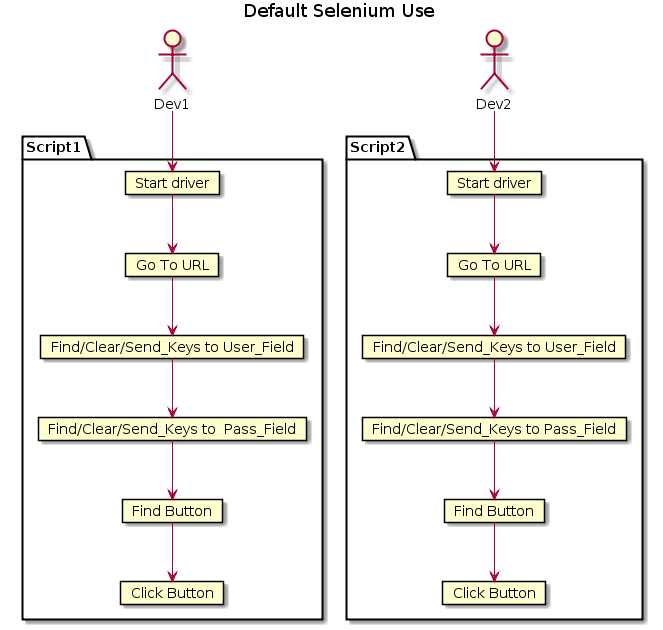
\includegraphics[width=1\textwidth]{./04-figuras/page_object_selenium}
        \label{fig:selenium_default}
    \end{figure}

    \begin{figure}[H]
        \vspace*{0,3cm}
        \centering
        \caption{Uso padrão Selenium com módulo}
        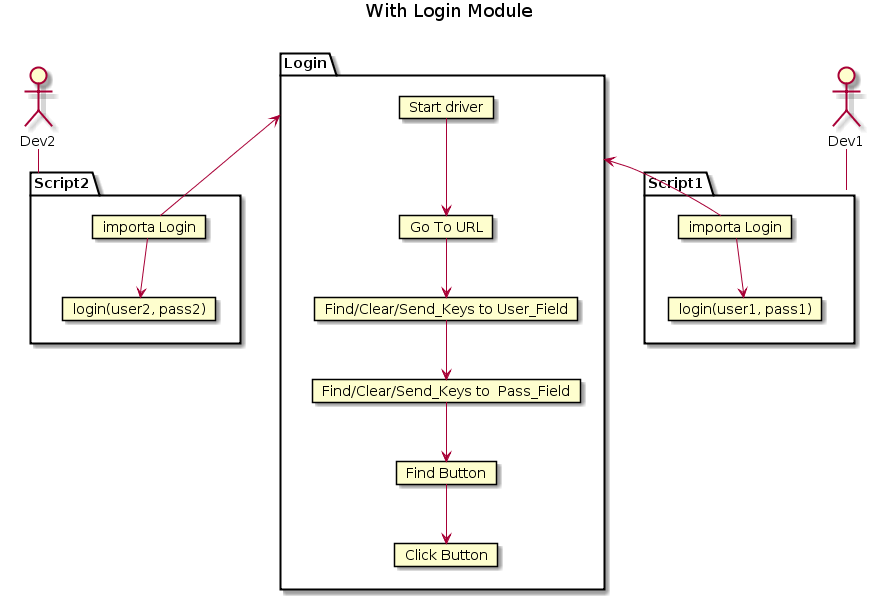
\includegraphics[width=1\textwidth]{./04-figuras/page_object_module}
        \label{fig:selenium_module}
    \end{figure}

    \begin{figure}[H]
        \vspace*{0,3cm}
        \centering
        \caption{Uso padrão Pybot}
        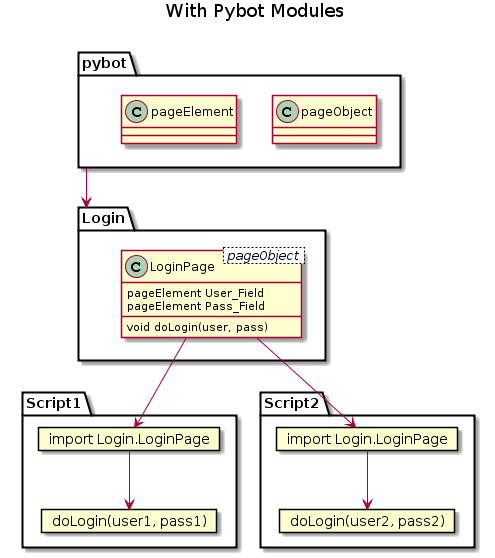
\includegraphics[width=1\textwidth]{./04-figuras/page_object_pybot}
        \label{fig:pybot_module}
    \end{figure}

\end{apendicesenv}